\chapter{简支梁平面问题的有限元解}
\label{cha:FEAsolution}
本章节使用商业有限元软件~ABAQUS~求解简支梁平面问题,即通过数值方法得到有限元解。对模型的信息和参数化建进行简述,并对计算得到的简支梁的应力、应变、位移场量进行分析和可视化。
\section{有限元模型的建立}
\subsection{单元类型选择}
在~ABAQUS~中,图\ref{fig:load}所示的简支梁可以使用梁单元(Beam Element)或实体单元(Solid Element)来模拟\cite{souza2014finite,frangi2010finite},如图\ref{fig:models}所示。
\begin{figure}[htbp]
    \centering
	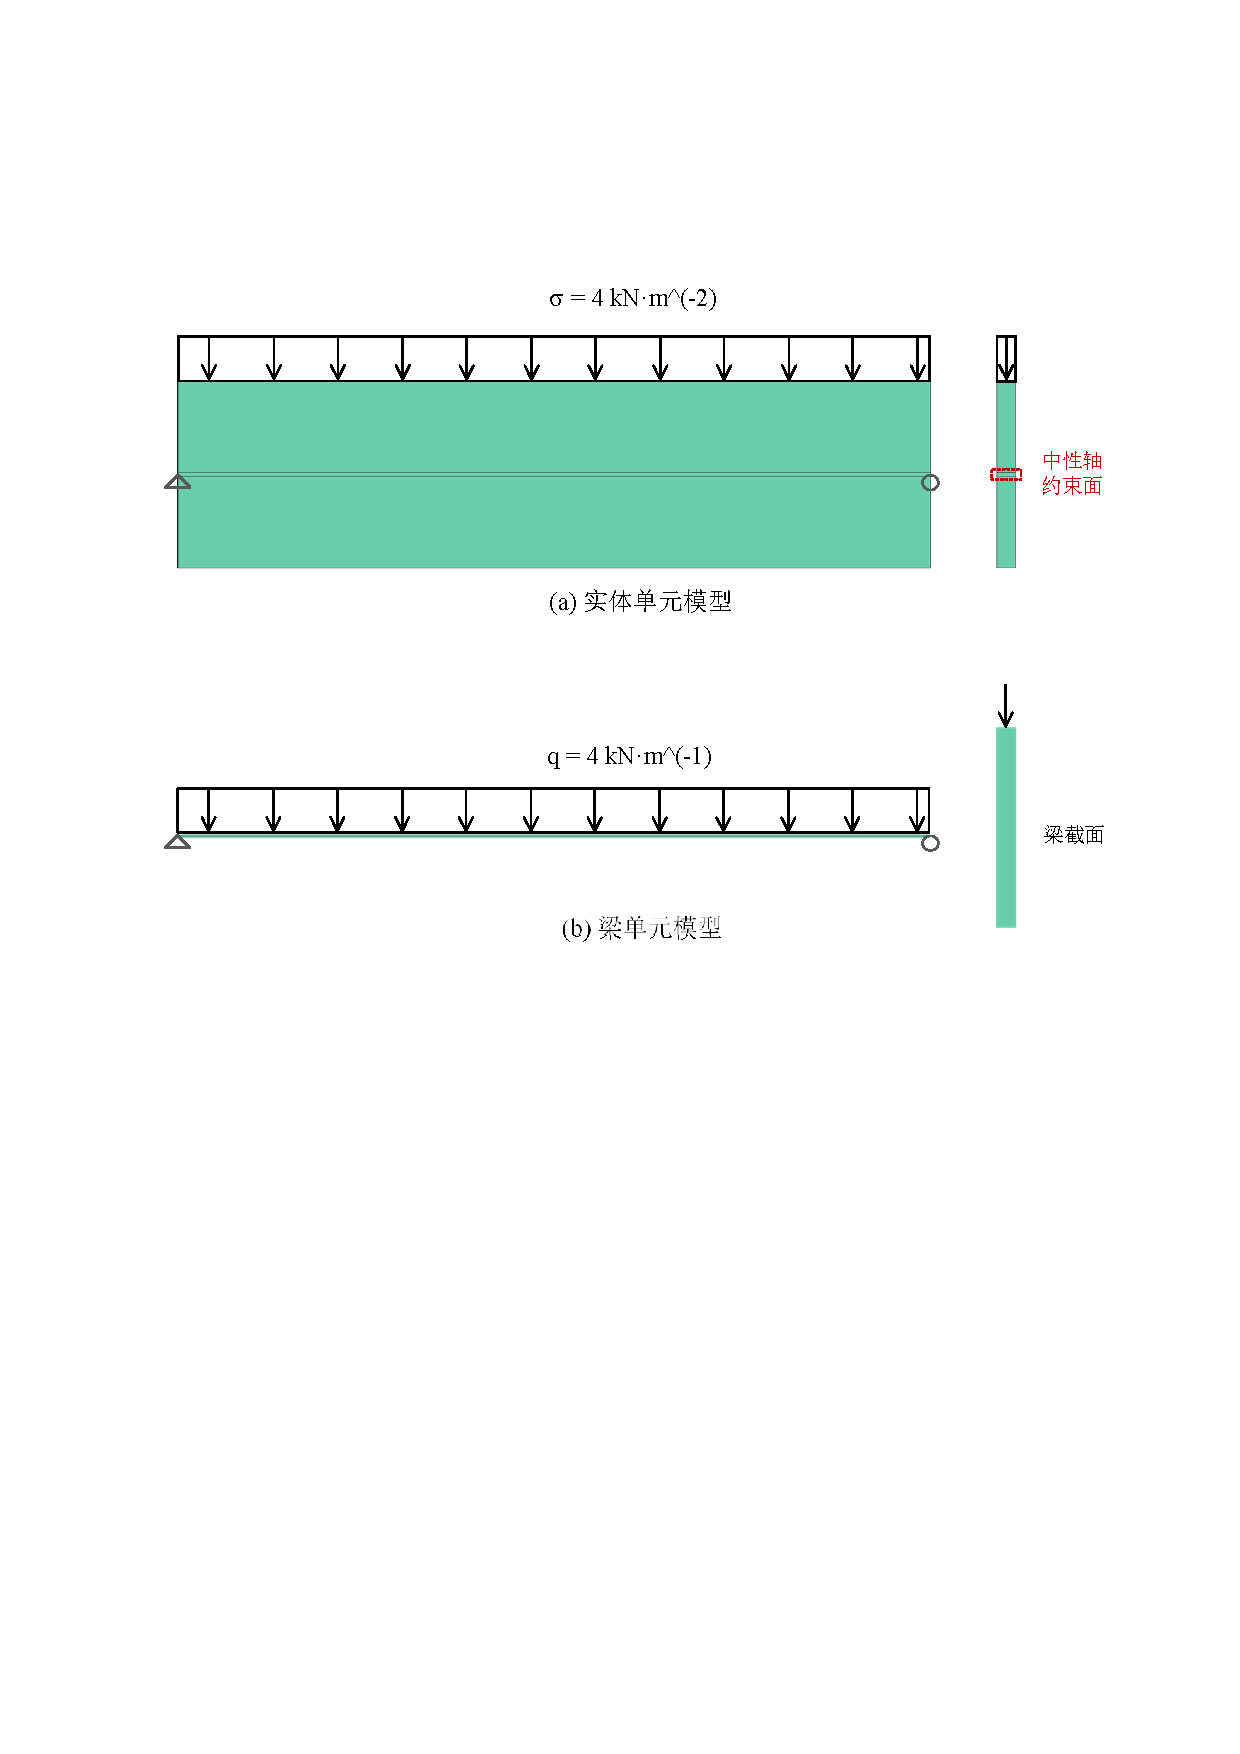
\includegraphics[width=1\textwidth]{figure3}
    \caption{ABAQUS中梁单元和实体单元模型}
    \label{fig:models}
\end{figure}
其中梁单元适用于分析中如果梁的横截面几何尺寸远小于其长度时的情况,能较好地模拟结构的整体变形,适和得出简支梁的位移分布。因为梁单元直接假设了梁的弯曲和拉伸行为,通过简化的刚度矩阵,能够快速、准确地反映结构的整体位移。它省略了横截面内部的应力细节,只提供关键的全局位移,降低了误差。
实体单元通过大量的网格划分来精确模拟简支梁,适用于任意形状的简支梁,能较好地模拟简支梁网格点处具体的应力、应变和位移分量并绘制云图。实体单元模型也能反应荷载施加点或约束处的应力集中问题\cite{belytschko2013nonlinear}。

因此本研究首先建立简支梁的实体单元模型,得出应力、应变、位移的有限元解,然后建立对应的梁单元模型,计算该模型下的位移有限元解,并讨论两种模型的计算误差。
\subsection{模型参数设置}
模型的形状参数与材料参数的设置与\ref{cha:visualization}章一致。但是三维有限元模型需要考虑梁的厚度(截面宽度)。在本章节先假定梁的厚度为~100~mm,下一章节对梁厚度的影响进行参数化分析。在网格划分模块中,实体单元模型选择~C3D8R~单元,最大网格尺寸设置为~20;梁单元模型选择~B31~单元,最大网格尺寸设置为~20,其余参数不变\cite{radon2015study},如图\ref{fig:mesh}所示。最后创建静力分析步并设置应力、应变和位移场输出\cite{liu2016review}。
\begin{figure}[htbp]
    \centering
	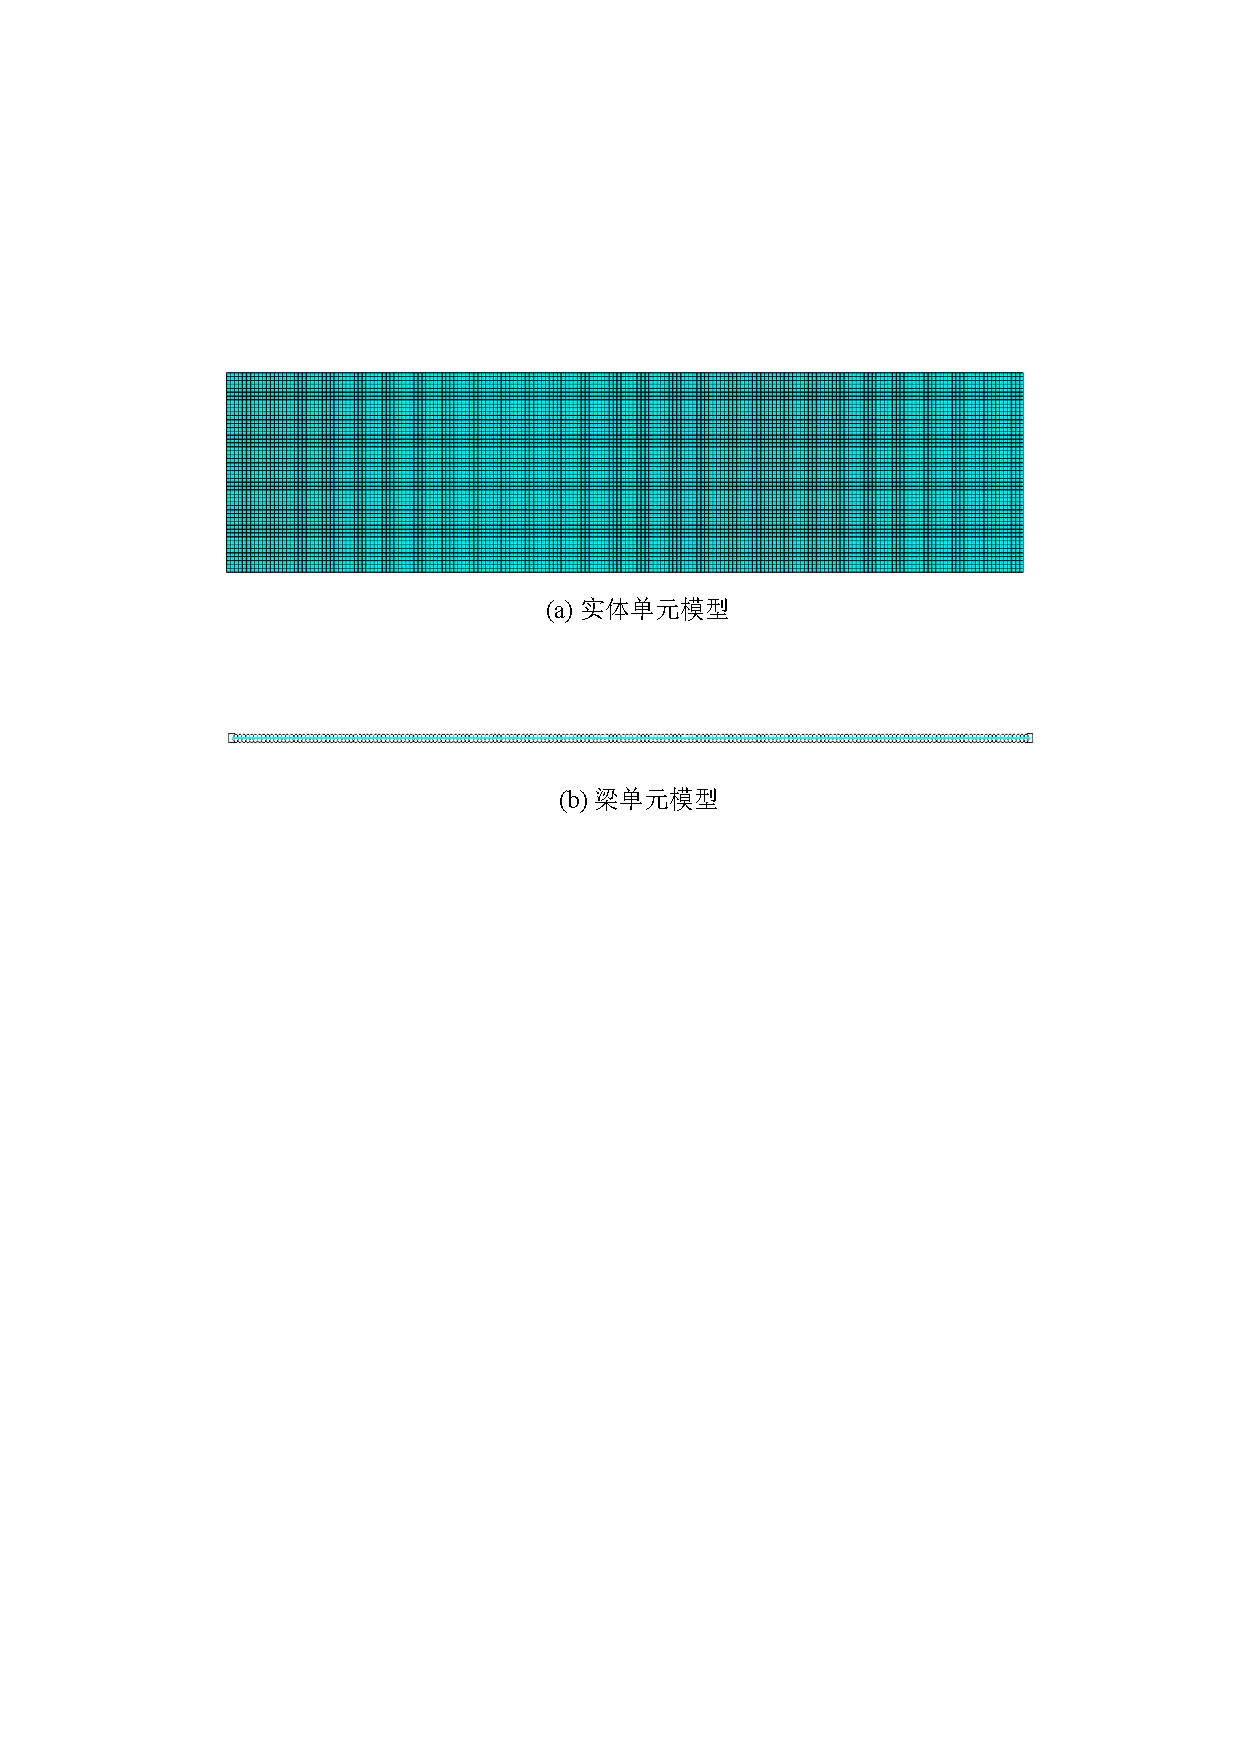
\includegraphics[width=1\textwidth]{figure5}
    \caption{网格划分}
    \label{fig:mesh}
\end{figure}
\subsection{边界条件设置}
简支梁的支座仅约束梁的垂直位移,梁端可自由转动。为使整个梁不产生水平移动,在一端加设水平约束,该处的支座称为铰支座,另一端不加水平约束的支座称为滚动支座。因此,在梁单元模型中,通过位移/转角约束,限制左端节点的~U1、U2、U3~分量,限制右端节点的~U1、U3~分量\cite{gajdosova2018influence},通过线荷载的形式施加均布荷载~4~N/mm;在实体单元模型中,对梁的中性面两侧单元进行约束\cite{JGXB201402012},同样限制左端节点的~U1、U2、U3~分量,限制右端节点的~U1、U3~分量,通过应力的形式施加均布荷载~4~MPa。将上述边界条件设置在静力分析步中,提交工况并得出结果。
\section{参数化建模}
为了探究~ABAQUS~中简支梁的厚度~$b$~对数值模拟结果的影响,将实体单元的模型信息转化为~python~代码,并对~$b$~进行单参数分析\cite{radon2015study,liu2016review}。在~BaseSolidExtrude~方法中,将参数~depth~设置为~1~和~20~至~200~等步长为~20~的共~11~个离散采样点\cite{fu2019recent}。将修改后的代码导入ABAQUS中,提交工况并得出结果。
\section{数值解的分析与讨论}
\subsection{参数分析}
参数分析得到的简支梁跨中最大弯曲应力和挠度随厚度变化的曲线如图\ref{fig:para}所示。
\begin{figure}[htbp]
    \centering
	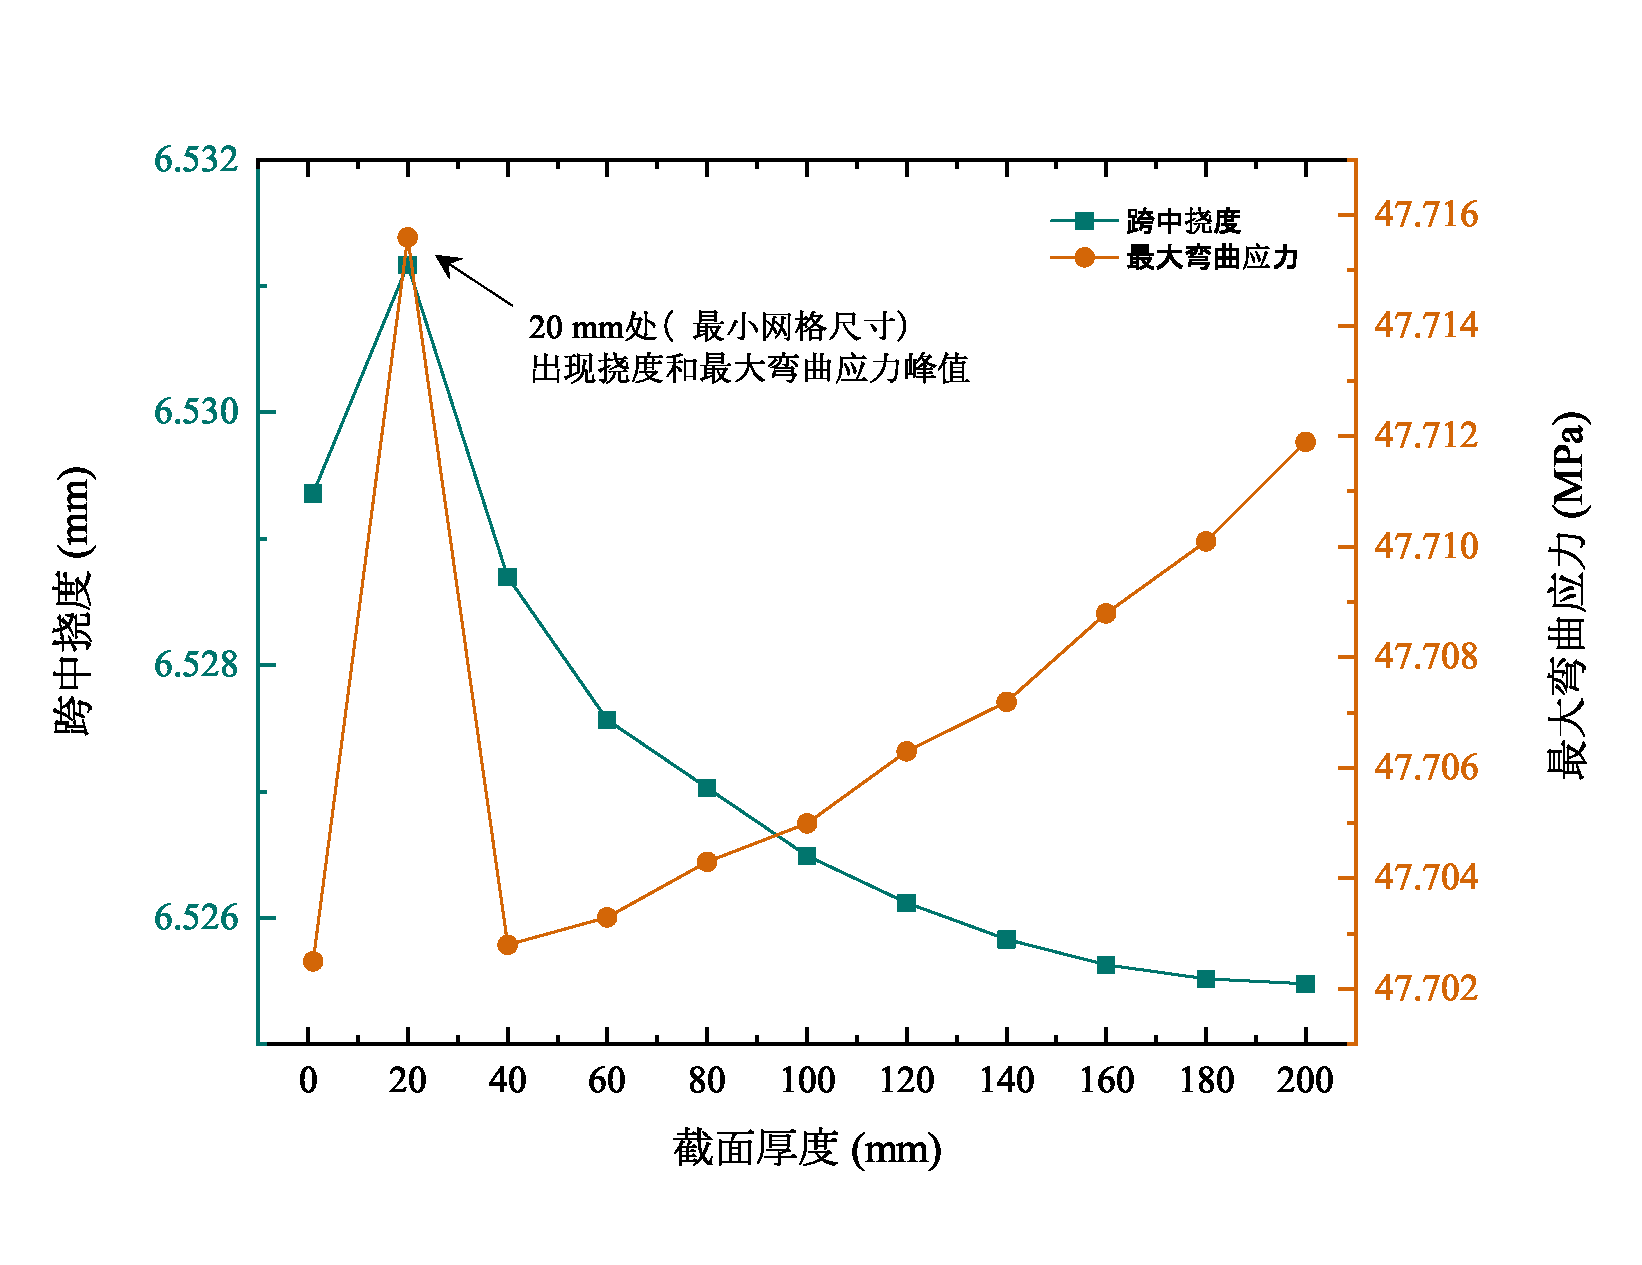
\includegraphics[width=1\textwidth]{figure6}
    \caption{最大弯曲应力和挠度与截面厚度的相关曲线图}
    \label{fig:para}
\end{figure}
结果表明,在设定的最大网格尺寸~20~mm~下,跨中挠度和最大弯曲应力均出现在简支梁厚度为~20~mm~处。当厚度小于~20~mm~时,挠度减小,最大弯曲应力减小;当厚度大于~20~mm~时,挠度逐渐减小,最大弯曲应力先减小,后逐渐增大。

\subsection{结果讨论}
实体单元模型的数值模拟结果如图\ref{fig:fea}所示。结果表明,(1)横向应力在梁的上下表面呈现明显的正负对称分布。上表面靠近中部区域出现最大拉应力,而下表面则呈现最大压应力。在梁的中心位置,即跨中,横向应力值相对较小,逐渐向两端边缘增大。纵向应力在非支座处沿高度方向分布较为均匀,且整体呈现负值,显示出梁的纵向受压状态,而在支座处出现了应力集中现象。剪应力分布具有左右正负对称性,在梁的两侧边缘达到最大,而在梁的跨中区域接近于零。(2)横向应变的分布与横向应力类似,梁的上下表面出现了明显的压应变和拉应变。纵向应变与应力的呈现形式不同,不沿高度方向均匀分布,主要受到泊松比和横向应力的影响,且靠近支座的边缘区域出现了应变集中。
\begin{figure}[htbp]
    \centering
	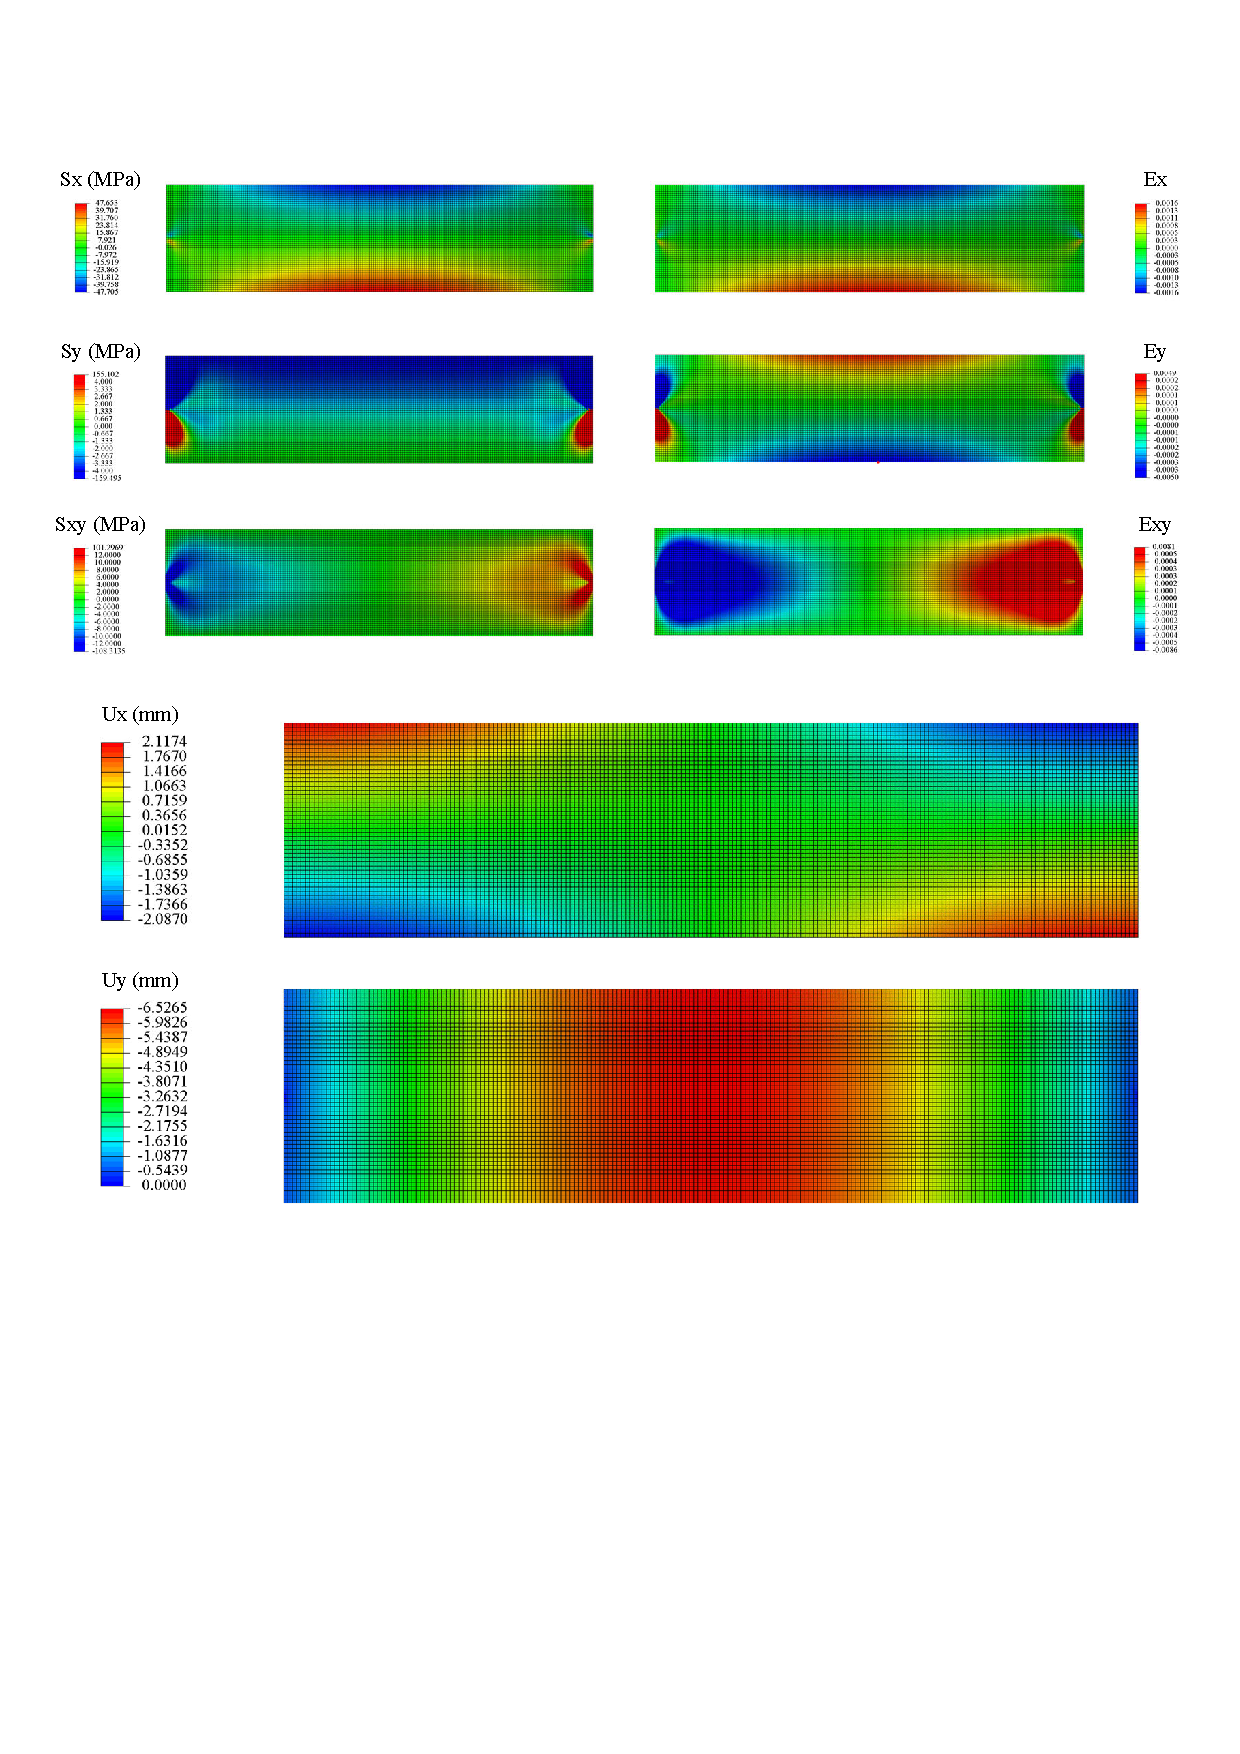
\includegraphics[width=1\textwidth]{figure4}
    \caption{实体单元模型数值模拟结果云图}
    \label{fig:fea}
\end{figure}
剪切应变与剪应力分布一致。(3)横向位移在梁的边缘区域达到最大值,且呈反对称分布。梁的中心区域横向位移接近于零,说明梁在两端的支座处发生了一定的转动。纵向位移从支座端开始逐渐增大,在跨中位置达到最大值。这种纵向位移分布表现出简支梁在均布荷载作用下的弯曲挠度特征,符合弯曲变形曲线的形状。

梁单元模型的数值模拟结果如图\ref{fig:BEAMfea}所示。结果表明,简支梁的挠度成抛物线状,与实体单元模型的挠度呈现相同的变化趋势。简支梁的弯曲应力左右对称,在跨中位置达到最大值。
\begin{figure}[htbp]
    \centering
	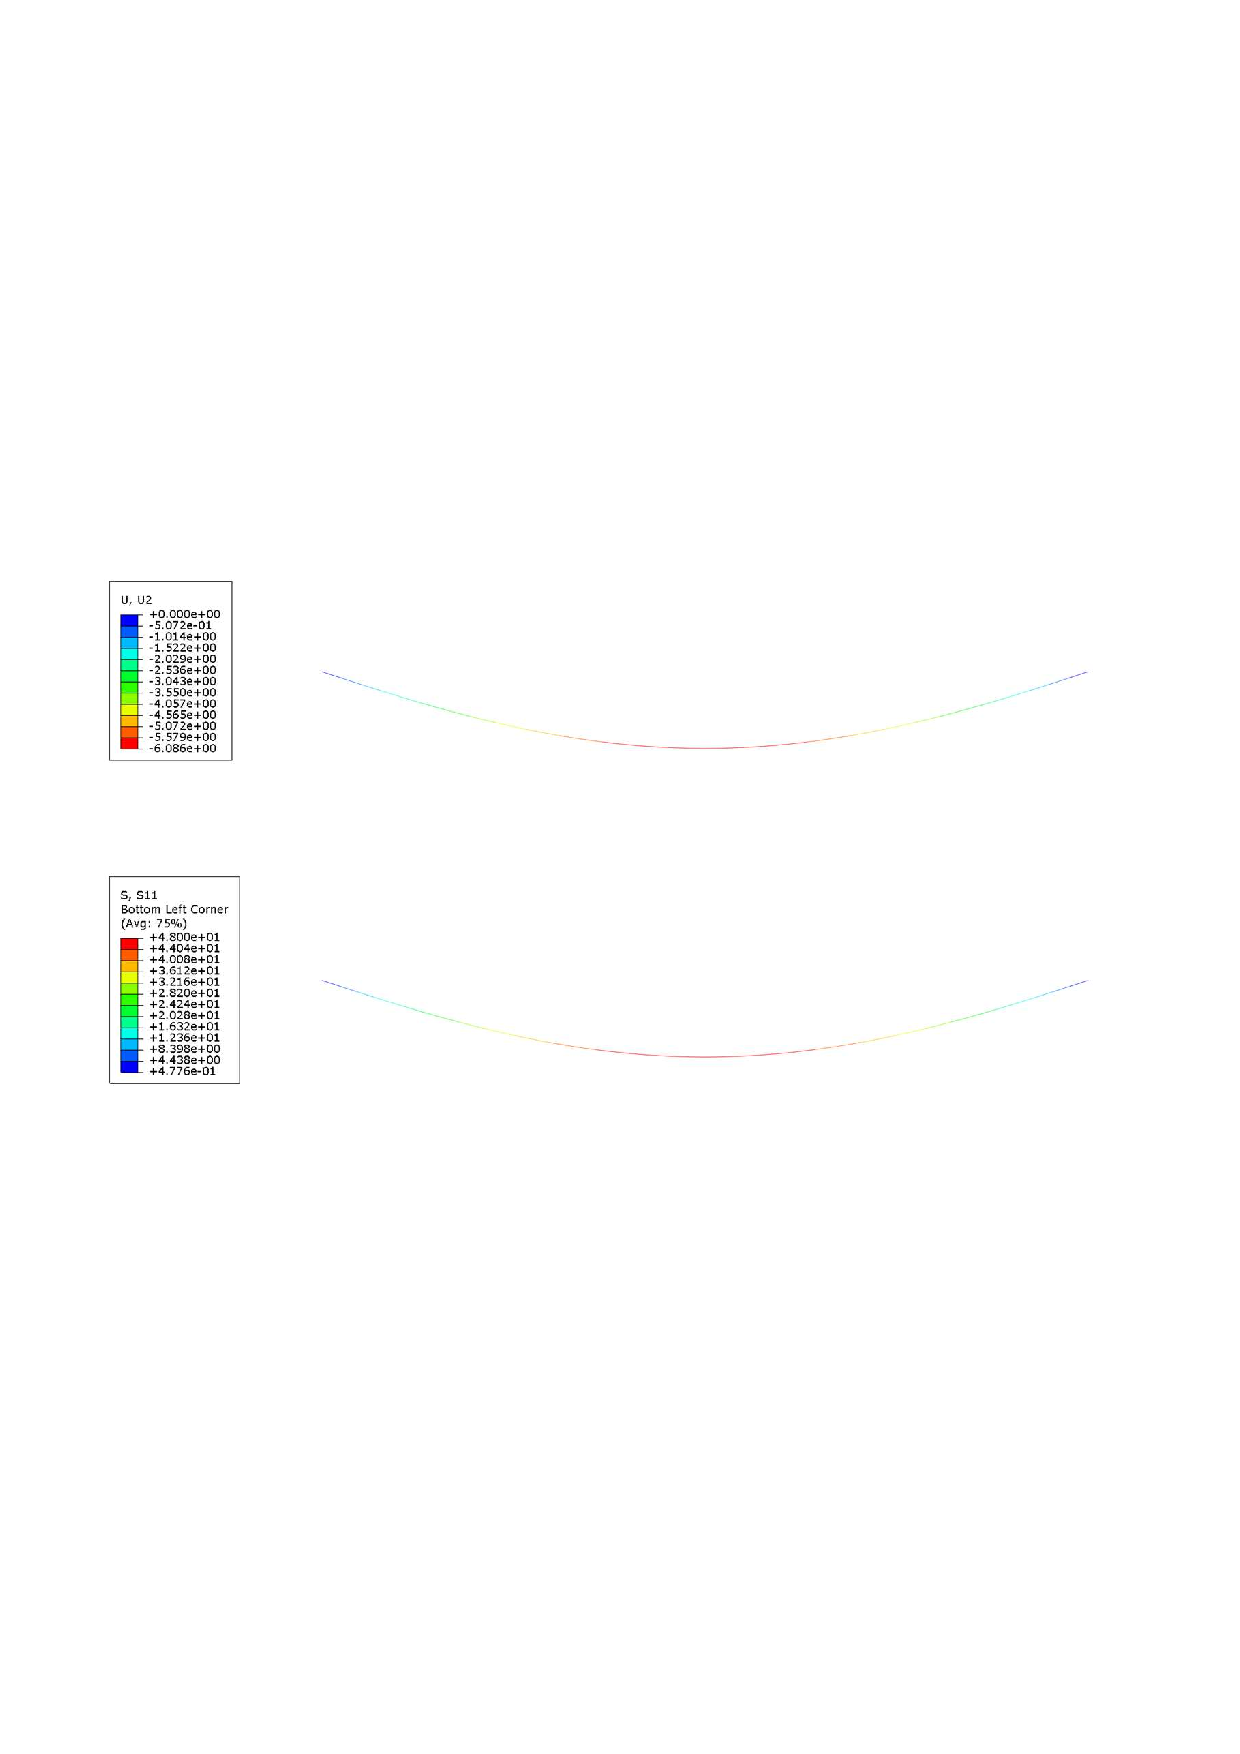
\includegraphics[width=1\textwidth]{figure7}
    \caption{梁单元模型数值模拟结果云图}
    \label{fig:BEAMfea}
\end{figure}

本章节,我们建立了简支梁的有限元模型,利用数值方法求解了上述问题的有限元解。梁单元采用简化的力学公式计算应力,而实体单元通过有限元方法逐步求解,因此在细节上存在微小差异如下。(1)梁单元主要考虑整体的弯曲行为,得出的最大挠度为~6.086~mm,而实体单元得出的最大挠度为~6.526~mm,偏大了约~7\%。(2)梁单元忽略了横截面内的应力细节,只能给出~Sx~的应力分布,而实体单元可以给出~Sy~和~Sxy~应力分布。其中梁单元给出的最大弯曲应力为~48.0~MPa,而实体单元给出的最大弯曲应力为~47.7~MPa,两者几乎一致(3)在支座约束处,实体单元能更好的体现刚性支座对梁两端网格自由度的约束。
